%----------------------------------------------------------------------------------------
% Preambulo y Configuración
%----------------------------------------------------------------------------------------
% command apply for end file pdflatex -synctex=1 -interaction=nonstopmode -jobname=mitesis %.tex
\documentclass[
    11pt,
    spanish,
    singlespacing,
    parskip,
    headsepline,
    bookmarks=true,
    unicode=true,
    pdftoolbar=true,
    pdfmenubar=true,
    pdffitwindow=false,
    colorlinks=true,
    linkcolor=blue,
    citecolor=blue,
    urlcolor=blue
]{MastersDoctoralThesis}

\usepackage[utf8]{inputenc} % Codificación de entrada UTF-8
\usepackage[T1]{fontenc}    % Codificación de salida para caracteres especiales
\usepackage{graphicx}       % Manejo de gráficos
\usepackage{eso-pic}        % Permite agregar fondos
\usepackage{hyperref}       % Manejo de hipervínculos y marcadores

% Redefinición de caracteres problemáticos en marcadores
\hypersetup{
    pdftitle={Gaston},
    pdfauthor={GastON VALDEZ},
    pdfkeywords={Sistemas Embebidos, Internet de las Cosas, Inteligencia Artificial},
    pdfstartview={FitH},
    unicode=true,
    colorlinks=true,
    linkcolor=blue,
    citecolor=blue,
    urlcolor=blue
}

\pdfstringdefDisableCommands{%
  \def\texttt#1{#1}%
  \def\textbf#1{#1}%
  \def\textit#1{#1}%
  \def\"{\"}%
  \def\~{~}%
  \def\'{'}%
  \def\^{}%
  \def\textunderscore{\_} % Manejo del subrayado en marcadores
}


% Definir comandos requeridos por la clase
\newcommand{\degreename}{Maestría en Ciencias} % Cambia según tu título
\newcommand{\univname}{Universidad Nacional de Ejemplo} % Cambia según tu universidad
\newcommand{\keywordnames}{Palabras clave:}
%----------------------------------------------------------------------------------------
% Documento Principal
%----------------------------------------------------------------------------------------

\begin{document}

% Configuración de la portada
\posgrado{Carrera / Maestría}
\keywords{Sistemas Embebidos, Internet de las Cosas, Inteligencia Artificial}
%\begin{flushleft}
%	\begin{center}
%		\begin{flushright}
%			este es un intendo de ver la compliaciones de compilar esta cosa ! 
%		\end{flushright}
%	\end{center}
%\end{flushleft}
% Incluir la portada desde un archivo separado
%----------------------------------------------------------------------------------------
% PORTADA
%----------------------------------------------------------------------------------------
\begin{titlepage}
	% Fondo completo con el PDF que incluye la barra y el logo
	\AddToShipoutPictureBG*{\includegraphics[width=\paperwidth, height=\paperheight]{Figures/fondo.pdf}}
	
	% Contenido principal
	\begin{flushright}
		\setlength{\rightskip}{-2cm} % Ajusta la sangría derecha
		\vspace*{7.5cm} % Ajustar según la posición vertical deseada
		
		% Título
		{\fontfamily{phv}\bfseries\fontsize{33pt}{40pt}\selectfont
			Control de actitud (ADCS)} \\[1.5cm]
		
		% Autor
		{\fontfamily{phv}\fontsize{20pt}{25pt}\selectfont
			Gastón Valdez} \\[1cm]
		
		% Carrera o Maestría (comentar o descomentar la línea correspondiente)
		{\fontfamily{phv}\fontsize{15pt}{20pt}\selectfont
			\textbf{Carrera de Especialización en Sistemas Embebidos}
			% \textbf{Carrera de Especialización en Internet de las Cosas} \\
			% \textbf{Carrera de Especialización en Inteligencia Artificial} \\
			% \textbf{Maestría en Sistemas Embebidos} \\
			% \textbf{Maestría en Internet de las Cosas} \\
			% \textbf{Maestría en Inteligencia Artificial Embebida} \\
			% \textbf{Maestría en Computación de Borde} \\
			% \textbf{Maestría en Inteligencia Artificial} \\
		} \\[2cm]
		
		% Director
		{\fontfamily{phv}\fontsize{11pt}{15pt}\selectfont
			\textbf{Director:} Amilcar Rincon Charris (UPM)} \\[1cm]
		
		% Jurados
		{\fontfamily{phv}\fontsize{11pt}{15pt}\selectfont
			\textbf{Jurados:}} \\[0.5cm]
		{\fontfamily{phv}\fontsize{11pt}{15pt}\selectfont
			Jurado 1 (pertenencia)} \\ 
		{\fontfamily{phv}\fontsize{11pt}{15pt}\selectfont
			Jurado 2 (pertenencia)} \\ 
		{\fontfamily{phv}\fontsize{11pt}{15pt}\selectfont
			Jurado 3 (pertenencia)} \\[2cm]
		
		% Fecha y lugar
		{\fontfamily{phv}\itshape\fontsize{10pt}{12pt}\selectfont
			Ciudad de La plata, Octubre de 2025} % Ejemplo: Ciudad de Córdoba, junio de 2025
	\end{flushright}
\end{titlepage}

% Configuración del contenido preliminar
\frontmatter % Usar numeración romana para las páginas preliminares
\pagestyle{plain} % Estilo de encabezado simple

%----------------------------------------------------------------------------------------
% Resumen
%----------------------------------------------------------------------------------------

\begin{abstract}
\addchaptertocentry{\abstractname} % Agregar resumen al índice
El resumen debe escribirse en uno o dos párrafos. Debe ser breve y conciso, sin ningún elemento de formato en el texto como itálicas o negritas. Tampoco se deben usar siglas ni acrónimos que no resulten obvios para un lector promedio de la memoria, ni referencias bibliográficas o notas al pie de página. No debe faltar qué es lo que se hizo/logró, qué importancia/valor tiene el proyecto/resultado, qué va a encontrar el lector en la memoria y qué contenidos de la especialización/maestría se aplicaron en el proyecto.
\end{abstract}

%----------------------------------------------------------------------------------------
% Agradecimientos
%----------------------------------------------------------------------------------------

\begin{acknowledgements}
\vspace{1.5cm}
Esta sección es para agradecimientos personales y es totalmente \textbf{OPCIONAL}.
\end{acknowledgements}

%----------------------------------------------------------------------------------------
% Índice
%----------------------------------------------------------------------------------------

\tableofcontents
\listoffigures
\listoftables

%----------------------------------------------------------------------------------------
% Dedicatoria
%----------------------------------------------------------------------------------------

\dedicatory{\textbf{Dedicado a... [OPCIONAL]}}

%----------------------------------------------------------------------------------------
% Capítulos
%----------------------------------------------------------------------------------------

\mainmatter % Iniciar numeración numérica para el contenido principal
\pagestyle{thesis} % Estilo de encabezado de tesis

% Incluir capítulos desde archivos separados
% Chapter 1

\chapter{Introducción general} % Main chapter title

\label{Chapter1} % For referencing the chapter elsewhere, use \ref{Chapter1} 
\label{IntroGeneral}
Un sistema de control de actitud\footnote{ADCS, por sus siglas en inglés \textit{Attitude Determination and Control System}} es un conjunto de componentes de hardware y software que permite a un satélite o nave espacial mantener o modificar su orientación en el espacio. Para realizar estos ajustes, el sistema utiliza \textbf{actuadores}\footnote{Dispositivo físico que genera movimiento o aplica fuerza para modificar la posición/orientación de un objeto.}. Su funcionamiento integra tres funciones clave:

\begin{enumerate}
	\item \textbf{Adquisición de datos}: Lectura de sensores (magnéticos, inerciales, etc.).
	\item \textbf{Procesamiento}: Estimación de la orientación mediante algoritmos.
	\item \textbf{Corrección}: Aplicación de fuerzas/torques mediante actuadores.
\end{enumerate}

Estas correcciones minimizan la diferencia entre la orientación actual y la deseada, garantizando precisión en aplicaciones como vehículos espaciales, drones o sistemas de estabilización.
%----------------------------------------------------------------------------------------

% Define some commands to keep the formatting separated from the content 
\newcommand{\keyword}[1]{\textbf{#1}}
\newcommand{\tabhead}[1]{\textbf{#1}}
\newcommand{\code}[1]{\texttt{#1}}
\newcommand{\file}[1]{\texttt{\bfseries#1}}
\newcommand{\option}[1]{\texttt{\itshape#1}}
\newcommand{\grados}{$^{\circ}$}

%----------------------------------------------------------------------------------------

%\section{Introducción}

%----------------------------------------------------------------------------------------
\section{Control de actitud}
En la actualidad existen pequeños satélites que orbitan alrededor de la tierra denominados CubeSats. Estos usan componentes electrónicos modulares y uno de ellos se llama ADCS. En la siguiente imagen puede verse un módulo comercial 
	\begin{figure}[htbp]
	\centering
	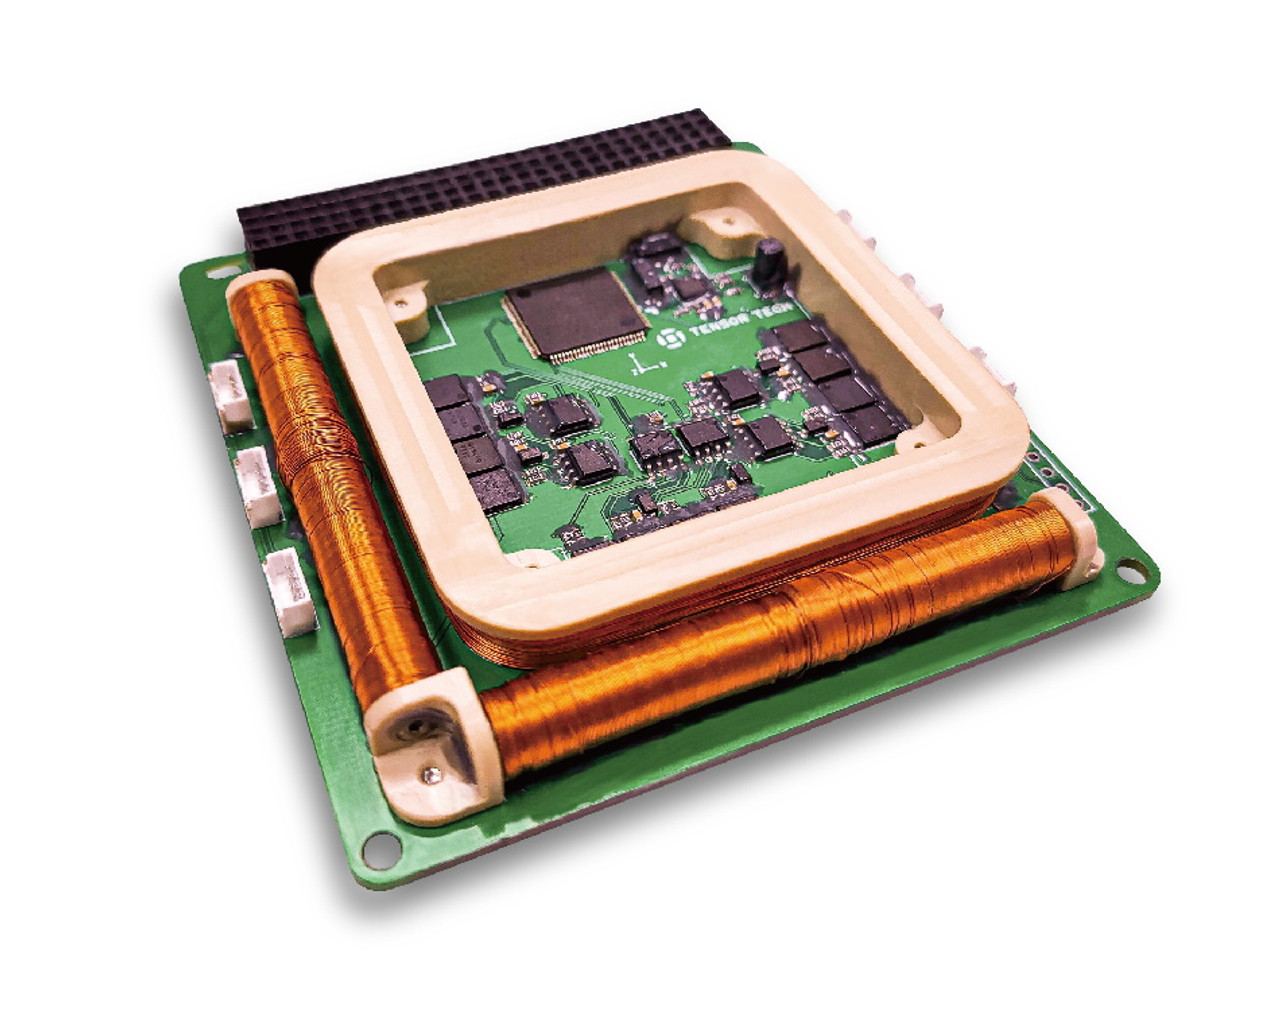
\includegraphics[width=0.5\textwidth]{./Figures/ADCS-Commercial.jpg}
	\caption{ADCS comercial - modelo ADCS-MTQ.}
	\label{fig:adcs_commercial}
\end{figure}


El sistema ADCS se encarga de mantener y corregir  la orientación del satélite a una orientación mediante un algoritmo de control. 

Un sistema ADCS consta de una unidad inercial de medición(IMU por sus siglas en inglés). Este dispositivo mide campo magnético, aceleración y velocidad angular en tres ejes. 
Con estos datos  determina la orientación dentro del espacio usando algoritmos como TRIAD, Davenports, entre otros.
Una vez calculada la orientación, el sistema genera una actuación (por ejemplo, mediante magnetorqueres o ruedas de reacción) para aplicar un torque (o par) en alguno de los ejes principales. Esto permite mantener la orientación deseada y compensar perturbaciones externas, como la resistencia atmosférica o la influencia gravitatoria. 


\section{Estado del Arte}

El control de actitud en vehículos espaciales es un área ampliamente estudiada, con múltiples enfoques que combinan sensores, algoritmos de estimación y actuadores para mantener o modificar la orientación del vehículo en el espacio. Existen diversas plataformas de simulación y validación de sistemas ADCS, muchas de ellas desarrolladas en entornos como MATLAB/Simulink, FreeFlyer, o STK. Sin embargo, estas soluciones presentan ciertas limitaciones, especialmente en contextos educativos o de bajo presupuesto.

Durante la etapa inicial de esta tesis se realizó una revisión exploratoria de herramientas disponibles, lo cual permitió identificar algunas dificultades frecuentes. Por un lado, muchas plataformas requieren licencias costosas, lo que puede restringir su uso en entornos académicos. Por otro, su complejidad técnica y curva de aprendizaje representan una barrera para estudiantes o investigadores que se inician en esta área. 

Además, se observó que pocas de estas herramientas permiten integración directa con microcontroladores u otros sistemas embebidos, lo cual complica la validación práctica de los algoritmos desarrollados. Del mismo modo, en varios casos la simulación de sensores se realiza bajo condiciones ideales, sin considerar la presencia de ruido, que limita la validez del modelo en entornos reales. 

Frente a estas limitaciones, el desarrollo propuesto en esta tesis busca ofrecer una alternativa accesible, de bajo costo y fácil de utilizar, que permita tanto la simulación como la conexión directa con hardware físico. Entre sus características, se destaca la capacidad de simular sensores con ruido, modificar algoritmos y configuraciones de sensores de manera modular, y validar los resultados directamente sobre un microcontrolador. Esto proporciona un entorno de desarrollo más realista y adaptable, especialmente útil en entornos educativos o de investigación aplicada. 



\section{Desarrollo del trabajo}
	El trabajo desarrolla la simulación de un control de actitud utilizando el algoritmo TRIAD para estimar la orientación del satelite. Este método compara dos referencias conocidas (por ejemplo campo magnético, aceleración de la gravedad, dirección del sol, etc) con las mediciones de los sensores a bordo. A partir de esta comparación,el TRIAD determina la orientación relativa del Cubesat respecto a un sistema de coordenadas de referencia. El diagrama en bloques del trabajo desarrollado se muestra a continuación: 
	\begin{figure}[htbp]
		\centering
		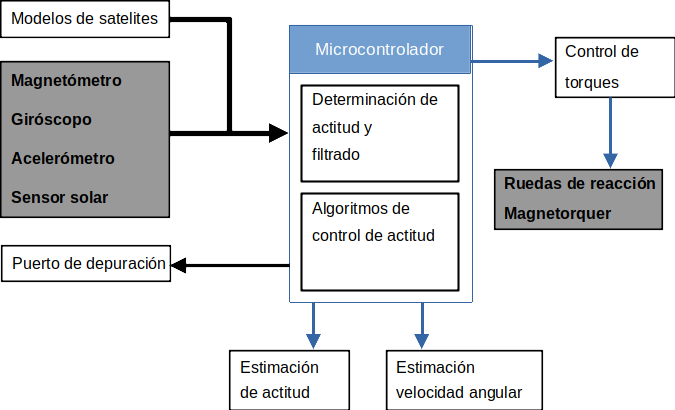
\includegraphics[width=0.7\textwidth]{./Figures/sistemaadcs.png}
		\caption{Diagrama en bloques del trabajo desarrollado.}
		\label{fig:simulate_sistem}
	\end{figure}

	El desarrollo de los algoritmos se realizó en dos lenguajes de programación: C para la implementación embebida y Python para prototipado rápido y validación de modelos. El código en C se integrará en un sistema embebido utilizando la metodología HIL (Hardware-in-the-Loop), que permite validar el comportamiento del sistema de control en un entorno simulado antes de su implementación física.





\section{Objetivos}

El objetivo inicial del proyecto consistía en desarrollar una placa de circuito impreso (PCB) con sistemas de actuación para control de actitud, ya sea mediante ruedas de reacción o magnetorquers. Sin embargo, durante la fase inicial de desarrollo se identificaron varias limitaciones significativas:

\begin{itemize}
	\item \textbf{Alto costo de soluciones comerciales}: Los modelos existentes para simulación presentaban costos prohibitivos para instituciones académicas.
	\item \textbf{Limitaciones en software libre}: Las herramientas analizadas (GMAT, Octave, entre otros) carecían de capacidad nativa para integración HIL (Hardware-in-the-Loop) con microcontroladores, siendo Matlab la única alternativa viable pero con sus propias dificultades técnicas.
	\item \textbf{Barreras económicas}: Los costos asociados a las soluciones comerciales resultaban inviables para su implementación en el contexto universitario.
\end{itemize}
Estos hallazgos motivaron una ampliación del alcance del trabajo, incorporando los siguientes objetivos tecnicos:

\begin{itemize}
	\item Desarrollo de un modelo dinámico de simulación que incluya:
	\begin{itemize}
		\item Modelado matemático del satélite y su entorno orbital
		\item Simulación de sensores (generación de datos sintéticos)
	\end{itemize}
	\item Implementación de una plataforma HIL que permita:
	\begin{itemize}
		\item Conexión con hardware real (microcontrolador/procesador)
		\item Inyección de datos de sensores simulados al sistema embebido
		\item Validación de los algoritmos de control en condiciones emuladas
	\end{itemize}
\end{itemize}


Este enfoque permitirá evaluar el rendimiento del sistema de control antes de proceder al diseño final del circuito impreso, reduciendo riesgos técnicos y costos asociados a iteraciones de hardware. Cabe aclarar que la simulación parte del supuesto de que el sistema ya se encuentra en la órbita deseada, sin modelar el proceso de inserción orbital ni el trayecto previo.





\chapter{Introducción específica} % Main chapter title

\label{Chapter2}

%----------------------------------------------------------------------------------------
%	SECTION 2 resume 
%----------------------------------------------------------------------------------------
Se presentan las bases matemáticas del control de actitud. El control de actitud se basa en seleccionar al menos dos sistemas de referencia para definir las orientaciones a través de una matriz. Al seleccionarse dos referencias puede utilizarse diferentes parametrizaciónes de la matriz: 
\begin{itemize}
	\item Quaterniones
	\item Parámetros de Rodrigues
	\item Parámetros de Euler
	\item Parámetros de Rodrigues modificado.
	\item etc,,, 
\end{itemize}
Esta parametrización presenta ventajas sobre la matriz. La idea central del control de actitud es estimar la matriz de orientaciones. EN este contexto la matriz se llama \"matriz de Actitude\". Esta matriz se obtiene a partir de la parametrización y del modelo dinámico del sistema, donde lo que se obtiene es una estimación y no la matriz real, según el algoritmo utilizado 
 

\section{Estilo y convenciones}
\label{sec:ejemplo}

\subsection{Rotaciones activas vs Pasivas}



\include{Chapters/Chapter3}
\include{Chapters/Chapter4}
\include{Chapters/Chapter5}

%----------------------------------------------------------------------------------------
% Apéndices
%----------------------------------------------------------------------------------------

\appendix

% Incluir apéndices desde archivos separados si es necesario
%\include{Appendices/AppendixA}

%----------------------------------------------------------------------------------------
% Bibliografía
%----------------------------------------------------------------------------------------

\renewcommand{\bibname}{Bibliografía} % Para asegurarte de que el título sea correcto
\phantomsection % Necesario para que el enlace del marcador sea correcto

\printbibliography[heading=bibintoc]

\end{document}






